\documentclass[a4paper]{article}
\pdfoutput=1
\usepackage{dblfloatfix}
\usepackage{caption}  
\usepackage{graphicx}
\usepackage[numbers]{natbib}
\usepackage{tikz}
\usetikzlibrary{shapes,arrows,calc,positioning}
\bibliographystyle{alpha}
\usepackage{amssymb}
\usepackage{amsmath}
\usepackage{mathtools}
\usepackage{algorithm}
\usepackage{algorithmicx}
\usepackage{algpseudocode}
\usepackage{subfigure}
\usepackage{paralist}
\usepackage{listings}
\usepackage{xcolor}
\usepackage[export]{adjustbox}
\usepackage{url}
\usepackage{csquotes}
\usepackage{color, colortbl}
\usepackage{mathdots}
\usepackage{tabularx}

\usepackage{amsthm}
\newtheorem{theorem}{Theorem}[subsection]
\newtheorem{lemma}[theorem]{Lemma}
\newtheorem{corollary}{Corollary}[theorem]
\newtheorem{definition}{Definition}[subsection]
\newtheorem{notation}{Notation}[subsection]
\newtheorem{remark}{Remark}[subsection]
\newtheorem{example}{Example}[subsection]

\lstset{language=C++,basicstyle=\ttfamily}

\begin{document}
\title{The Fractal Nature of Algorithms}
\author{Norbert~B\'atfai\\batfai.norbert@inf.unideb.hu\\Department of Information Technology\\University of Debrecen}

\maketitle

\begin{abstract}
Alan Turing had created a universal algorithm that can simulate all other algorithms. 
John von Neumann had constructed an automata that can reconstruct itself. 
In this paper we give a learning Turing machine that can learn any halting Turing machines. 
The main goal is to create a definition for machine learning that will be able to capture the properties of living systems described by Erwin Schrödinger.
\end{abstract}

\section{Introduction}

\cite{Turing}
\cite{Neumann}
\cite{TheorRobopsy}
\cite{WhatIsLife}

\begin{figure}[!h]
\centering
\scalebox{1}{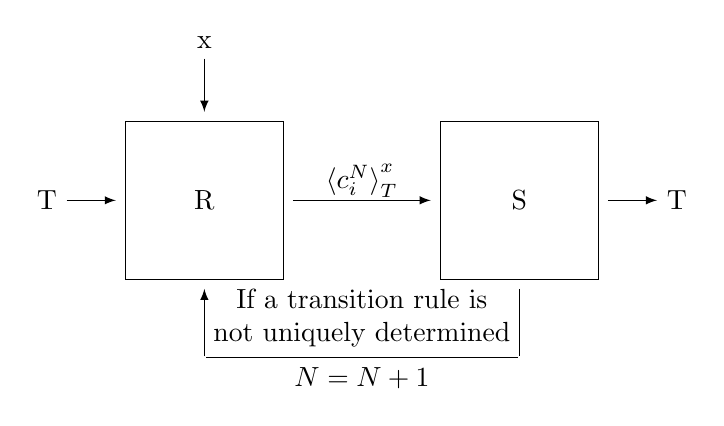
\begin{tikzpicture}

\draw  (-4,3.5) rectangle (-2,1.5);
\draw  (0,3.5) rectangle (2,1.5);
\node (v2) at (-5,2.5) {T};
\node (v1) at (-4,2.5) {};
\node (v4) at (-2,2.5) {};
\node (v3) at (0,2.5) {};
\node (v6) at (2,2.5) {};
\node (v5) at (3,2.5) {T};
\draw [-latex] (v2) edge (v1);
\draw [-latex] (v4) edge (v3);
\draw [-latex] (v6) edge (v5);
\node (v7) at (-3,3.5) {};
\node (v8) at (-3,4.5) {x};
\draw [-latex] (v8) edge (v7);
\node at (-3,2.5) {R};
\node at (1,2.5) {S};
\node at (-1,2.75) {${\langle c_i^N\rangle}_T^x$};
\node at (3,2.5) {};
\node  (v9) at (1,1.5) {};
\node [inner sep=0,outer sep=0](v10) at (1,0.5) {};
\node [inner sep=0,outer sep=0](v11) at (-3,0.5) {};
\node (v12)at (-3,1.5) {};

\draw (v9) edge (v10);
\draw (v10) edge (v11);
\draw  [-latex] (v11) edge (v12);

\node[align=center, below] at (-1,1.5) {If a transition rule is\\not uniquely determined};

\node[below] at (-1,0.5) {$N = N + 1$};
\end{tikzpicture}}
\caption{This figure shows the architecture of a universal learning machine.\label{fig_ULM}}
\end{figure}

\section{Conclusion}

\section{Acknowledgment}

\bibliography{AlgFract}

\end{document}